% ============================================================================
\section{Validación}\label{sec:validacion}
% ============================================================================

Fijados los parámetros (tabla~\ref{tab:config}), cada metaheurística se ha ejecutado
\emph{una sola vez} sobre las 24 instancias de \cod{Validacion\_datos/}, con las mismas 3
semillas y el mismo límite de 5 segundos: 360%
 ejecuciones.
Ningún parámetro se ha modificado después. La pregunta que responde esta sección es la de la
sección~\ref{sec:protocolo}: \emph{¿funcionan los parámetros elegidos igual de bien en
instancias que no han intervenido en su elección?}

\subsection{Calibración frente a validación}

\begin{table}[H]
\centering
\caption{Calibración frente a validación. RPD (\%) respecto del óptimo de la configuración final de cada algoritmo: media en las 6 instancias de calibración y media, desviación típica, mínimo y máximo sobre las ejecuciones en las 24 instancias de validación. Las dos últimas columnas son el número medio de columnas de la solución y el instante medio en que se encontró la mejor solución, en validación.}
\label{tab:validacion}
\begin{tabular}{@{}lrrrrrrr@{}}
\toprule
 & Calibración & \multicolumn{6}{c}{Validación} \\
\cmidrule(lr){2-2}\cmidrule(l){3-8}
Algoritmo & Media & Media & Desv. & Mín. & Máx. & Columnas & $t_{\text{mejor}}$ (s) \\ \midrule
Constructivo voraz & 6.596 & 6.448 & 0.738 & 5.167 & 7.622 & 166 & --- \\
Búsqueda local ($j_A=3$) & 4.817 & 4.665 & 0.539 & 3.816 & 6.073 & 139 & --- \\
\midrule
Temple Simulado & 4.127 & 4.067 & 0.344 & 3.131 & 4.910 & 149 & 3.75 \\
Búsqueda Tabú & 4.095 & 4.109 & 0.438 & 3.231 & 4.932 & 128 & 1.13 \\
GRASP & 3.441 & 3.448 & 0.312 & 2.639 & 4.206 & 130 & 4.32 \\
Algoritmo Genético & 4.292 & 4.275 & 0.452 & 3.112 & 5.298 & 144 & 4.51 \\
VNS & 3.585 & 3.521 & 0.451 & 2.435 & 4.499 & 124 & 3.90 \\
\bottomrule
\end{tabular}
\end{table}


\begin{figure}[H]\centering
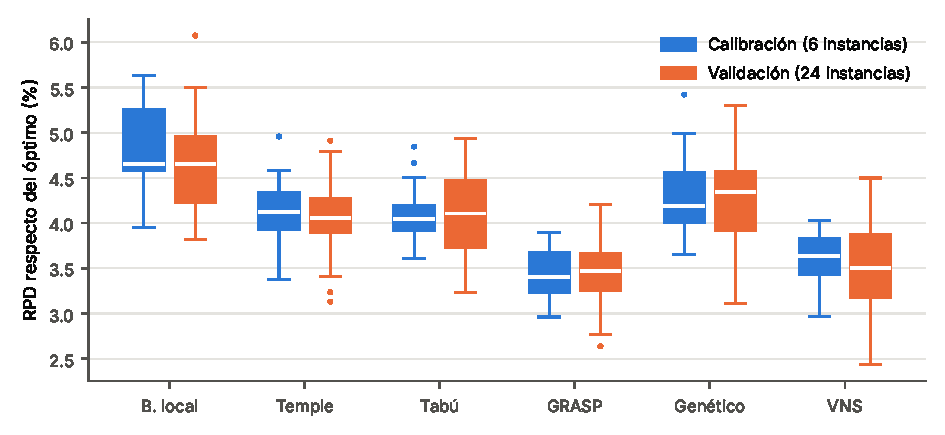
\includegraphics[width=0.86\textwidth]{figuras/validacion.pdf}
\caption{Distribución del RPD de todas las ejecuciones de la configuración final en las
instancias de calibración (18 ejecuciones por algoritmo) y de validación (72). La caja abarca
del primer al tercer cuartil; la línea blanca es la mediana.}
\label{fig:validacion}
\end{figure}

Lectura de la tabla~\ref{tab:validacion} y de la figura~\ref{fig:validacion}:
\begin{itemize}
  \item \textbf{No hay sobreajuste.} El RPD medio en validación es prácticamente igual al de
        calibración en los cinco algoritmos: la mayor diferencia es de seis centésimas
        (temple y VNS, y además a favor de la validación) y en GRASP y en la búsqueda tabú no
        llega a dos. Son diferencias menores que el propio ruido entre semillas.
  \item \textbf{La referencia confirma la lectura.} El constructivo y la búsqueda local no
        tienen nada que sobreajustar y, sin embargo, salen unas 15 centésimas mejor en las
        instancias de validación que en las de calibración: las 24 instancias de validación
        son, de media, ligerísimamente más fáciles. Las metaheurísticas se mueven menos que
        eso entre un conjunto y otro.
  \item \textbf{El orden entre algoritmos se mantiene.} En ambos conjuntos: GRASP, VNS,
        temple y tabú (empatados), genético, búsqueda local y constructivo. Lo único que
        cambia es el orden interno de la pareja temple--tabú, que están a cuatro centésimas.
  \item \textbf{La dispersión es parecida} en ambos conjuntos (figura~\ref{fig:validacion});
        en validación los extremos son algo más amplios simplemente porque hay cuatro veces
        más ejecuciones.
\end{itemize}

\begin{idea}[Conclusión de la validación]
Los parámetros elegidos con 6 instancias funcionan igual en las otras 24. La calibración es
válida para esta familia de instancias, y las cifras de validación (tabla~\ref{tab:validacion})
son las que deben usarse en el informe como estimación de la calidad de cada algoritmo.
\end{idea}

\paragraph{Una salvedad sobre el tiempo.} La validación se ejecutó en una sesión de cálculo
distinta de la calibración, en una máquina del mismo modelo que resultó en torno a un 10\,\%
más rápida (más iteraciones en los mismos 5 segundos). El efecto sobre el RPD es muy pequeño
porque al final de la ejecución todos los algoritmos mejoran ya muy despacio
(figura~\ref{fig:convergencia}), pero es una razón más para que, al repetir los experimentos,
calibración y validación se hagan seguidas en el mismo ordenador.

\subsection{Resultados por instancia}

\begin{table}[H]
\centering
\caption{Validación, instancia a instancia: valor óptimo y RPD (\%) de cada algoritmo (en las metaheurísticas, media de 3 semillas). En negrita, el mejor de cada fila.}
\label{tab:validacion-inst}
\small
\begin{tabular}{@{}lrrrrrrrr@{}}
\toprule
Instancia & Óptimo & Voraz & B. local & Temple & Tabú & GRASP & Genético & VNS \\ \midrule
SCP02 & 348.4449 & 6.69 & 4.92 & 4.34 & 4.68 & \textbf{3.48} & 4.54 & 3.73 \\
SCP03 & 360.7409 & 7.57 & 5.34 & 4.40 & 4.59 & \textbf{3.77} & 4.57 & 3.90 \\
SCP04 & 344.5675 & 5.59 & 4.23 & 4.07 & 3.65 & 3.37 & 4.17 & \textbf{3.30} \\
SCP05 & 347.3748 & 5.17 & 4.05 & 4.11 & 3.55 & 3.15 & 3.70 & \textbf{3.08} \\
SCP07 & 353.0618 & 6.09 & 4.74 & 4.20 & 4.31 & \textbf{3.69} & 4.61 & 3.84 \\
SCP08 & 351.9831 & 6.13 & 3.90 & 3.72 & 3.70 & 3.52 & 3.86 & \textbf{3.13} \\
SCP09 & 361.6024 & 6.65 & 4.44 & 4.06 & 4.10 & \textbf{3.46} & 4.22 & 3.51 \\
SCP10 & 362.9863 & 6.03 & 4.66 & 4.14 & 3.99 & \textbf{3.40} & 4.44 & 3.44 \\
SCP12 & 359.2725 & 6.07 & 4.65 & 4.00 & 4.39 & \textbf{3.27} & 4.39 & 3.47 \\
SCP13 & 350.6093 & 6.64 & 4.22 & 3.98 & 3.59 & 3.22 & 4.05 & \textbf{3.06} \\
SCP14 & 362.8942 & 7.28 & 5.15 & 3.99 & 4.21 & \textbf{3.29} & 4.27 & 3.62 \\
SCP15 & 351.7930 & 5.72 & 4.05 & 3.70 & 3.81 & \textbf{3.00} & 3.75 & 3.16 \\
SCP17 & 387.6437 & 7.22 & 5.50 & 4.34 & 4.51 & \textbf{3.80} & 4.85 & 4.36 \\
SCP18 & 379.7808 & 7.37 & 4.86 & 4.19 & 3.99 & 3.60 & 4.99 & \textbf{3.38} \\
SCP19 & 359.4288 & 5.82 & 4.87 & 3.76 & 4.04 & \textbf{3.00} & 4.17 & 3.36 \\
SCP20 & 362.8615 & 6.10 & 4.51 & 4.27 & 4.02 & 3.73 & 4.59 & \textbf{3.29} \\
SCP22 & 323.4298 & 5.97 & 4.21 & 3.30 & 3.67 & 3.13 & 3.65 & \textbf{2.80} \\
SCP23 & 363.8613 & 6.25 & 4.47 & 4.25 & 4.37 & \textbf{3.75} & 4.26 & 3.86 \\
SCP24 & 375.1956 & 7.02 & 5.21 & 3.93 & 4.52 & \textbf{3.45} & 4.55 & 3.99 \\
SCP25 & 362.9379 & 7.62 & 6.07 & 4.44 & 4.77 & 3.87 & 4.32 & \textbf{3.79} \\
SCP27 & 342.9086 & 5.72 & 3.82 & 3.88 & 3.27 & 3.45 & 3.92 & \textbf{3.04} \\
SCP28 & 321.7658 & 5.29 & 4.24 & 3.53 & 3.58 & 2.98 & 3.32 & \textbf{2.91} \\
SCP29 & 378.2595 & 7.24 & 5.07 & 4.26 & 4.80 & \textbf{3.63} & 4.52 & 4.24 \\
SCP30 & 377.9067 & 7.49 & 4.82 & 4.75 & 4.50 & \textbf{3.73} & 4.86 & 4.24 \\
\midrule
Media & & 6.45 & 4.67 & 4.07 & 4.11 & 3.45 & 4.27 & 3.52 \\
Veces mejor & & 0 & 0 & 0 & 0 & 14 & 0 & 10 \\
\bottomrule
\end{tabular}
\end{table}


La tabla~\ref{tab:validacion-inst} muestra que las conclusiones no dependen de unas pocas
instancias:
\begin{itemize}
  \item En las 24 instancias el mejor algoritmo es GRASP (14 veces) o la VNS (10 veces). La
        diferencia media entre ambos, siete centésimas a favor de GRASP, no es
        estadísticamente significativa (prueba de Wilcoxon de rangos con signo sobre las 24
        instancias, $p=0.32$): \textbf{GRASP y VNS están empatados}.
  \item La VNS es mejor que el temple en 22 de las 24 instancias y mejor que la búsqueda tabú
        en las 24; la diferencia (medio punto) sí es significativa ($p<0.001$).
  \item Temple y tabú están empatados entre sí ($p=0.53$) y ambos son algo mejores que el
        genético (dos décimas; $p<0.03$).
  \item GRASP, VNS y tabú mejoran a la búsqueda local en las 24 instancias y en sus 72
        ejecuciones; el temple, en 66 de 72; el genético, en 58 de 72.
\end{itemize}

\subsection{Evolución con el tiempo}

\begin{figure}[H]\centering
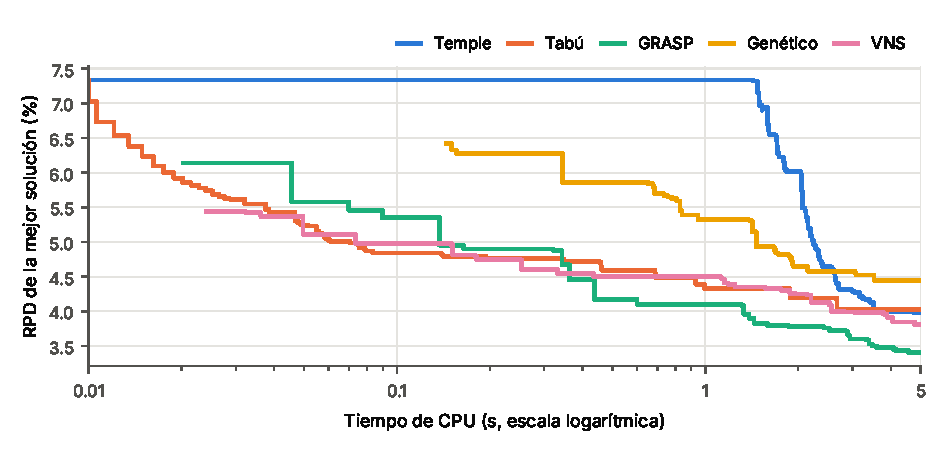
\includegraphics[width=0.86\textwidth]{figuras/convergencia.pdf}
\caption{Evolución del RPD de la mejor solución durante una ejecución de 5 segundos (instancia
SCP01, semilla 1, configuraciones finales). El eje de tiempos es logarítmico.}
\label{fig:convergencia}
\end{figure}

La figura~\ref{fig:convergencia} ilustra el comportamiento típico de cada algoritmo (es una
sola ejecución, no una media):
\begin{itemize}
  \item La \textbf{búsqueda tabú} y la \textbf{VNS} mejoran muy deprisa al principio: en una
        décima de segundo ya están en torno al 5\,\%. La tabú se estanca hacia la mitad de
        la ejecución; la VNS sigue encontrando mejoras pequeñas hasta el final.
  \item El \textbf{temple} no mejora nada durante el primer segundo y medio (fase caliente:
        acepta casi todo y la mejor solución sigue siendo la inicial) y después baja de
        golpe cuando la temperatura llega a la zona útil. Es el comportamiento esperado y
        explica por qué es tan sensible a la velocidad de enfriamiento.
  \item \textbf{GRASP} avanza a escalones cada vez más rentables: cuanto más pesa la memoria,
        mejores son las soluciones que construye. Sigue mejorando al final.
  \item El \textbf{genético} es el más lento en arrancar (tiene que construir la población),
        mejora de forma gradual durante toda la ejecución y termina por encima de los demás.
\end{itemize}
